\documentclass [12pt, a4paper] {article}
\usepackage[utf8x]{inputenc}
\usepackage[english,russian]{babel}
\usepackage[T2A]{fontenc}
\usepackage {graphicx}
\let\stdsection\section
\renewcommand\section{\newpage\stdsection}
\addto\captionsrussian{% Replace "english" with the language you use
  \renewcommand{\contentsname}%
    {Оглавление}%
}
\hypersetup{
    colorlinks,
    allcolors=blue
}

\begin {document}

\thispagestyle {empty}

\begin {center}
\ \vspace{-4cm}

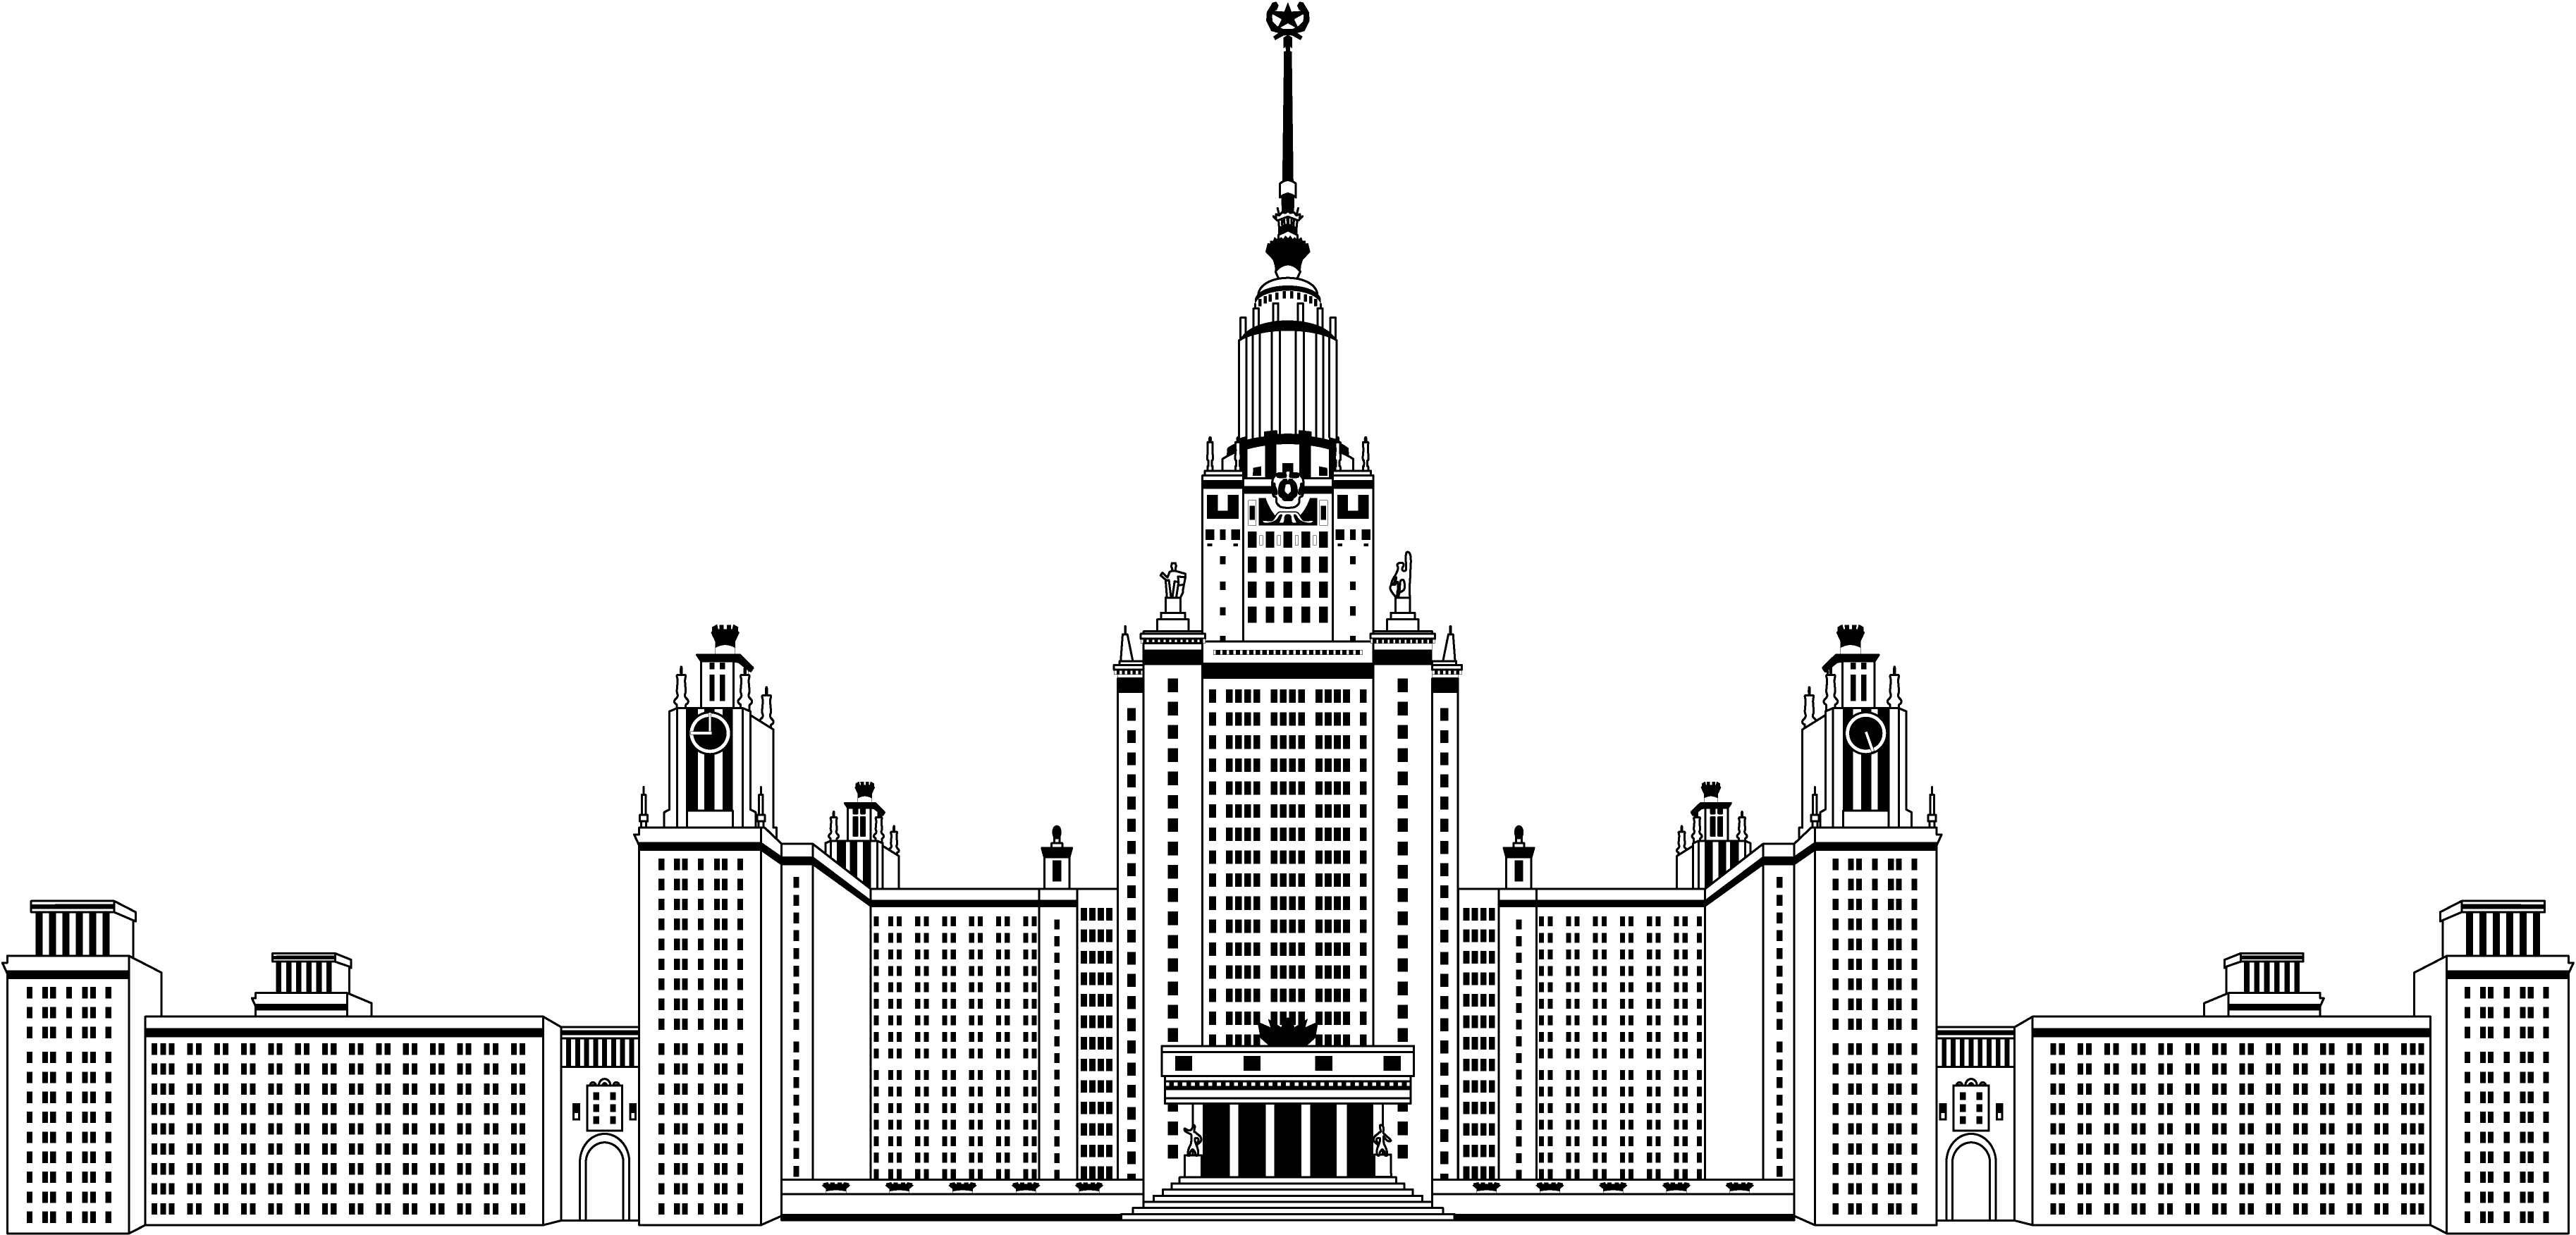
\includegraphics [width = 0.5 \textwidth] {msu.png} \\
{\scshape Московский Государственный Университет} \\
Факультет вычислительной математики и кибернетики\\

\vspace {5cm}

{\LARGE Essay}

\vspace {1cm}

{\Huge \bfseries
<<Джон Нэш и его вклад в теорию игр>> \\}
\end {center}

\vfill
\vfill

\begin {flushright}
  \large
  Гордеев Михаил \\
  студент группы 618/1 \\

  \vspace {5mm}
\end {flushright}

\vfill

\begin {center}
Москва, 2016
\end {center}

\enlargethispage {4 \baselineskip}

\newpage

\end {document}
